\documentclass[11pt,a4paper]{article}
\usepackage{nabiadoc}
\usepackage{tabularx}
\usepackage{caption}
\usepackage{tikz}
\usetikzlibrary{positioning,arrows.meta,fit}
\captionsetup[lstlisting]{justification=raggedright, singlelinecheck=false, font=small, labelfont=bf}

% Languages listings does not know.
\lstdefinelanguage{yaml}{sensitive=true, comment=[l]{\#}, morestring=[b]", morestring=[b]',
  keywords={true,false,null}}
\lstdefinelanguage{toml}{sensitive=true, comment=[l]{\#}, morestring=[b]", morestring=[b]',
  keywords={true,false}}
\lstdefinelanguage{PowerShell}{sensitive=false, comment=[l]{\#}, morecomment=[s]{<\#}{\#>},
  morestring=[b]", morestring=[b]',
  keywords={param,if,else,elseif,foreach,throw,try,finally,function,return}}
\lstdefinelanguage{cmake}{sensitive=false, comment=[l]{\#}, morestring=[b]",
  keywords={if,else,endif,install,set,find_package,pybind11_add_module,target_link_libraries,set_target_properties}}
\lstset{basicstyle=\ttfamily\scriptsize, captionpos=t, aboveskip=8pt, belowskip=8pt, tabsize=4,
        keepspaces=true, breaklines=true, postbreak=\mbox{\textcolor{gray}{$\hookrightarrow$}\space}}
\renewcommand{\lstlistingname}{File}

% A piece of a real file, extracted at build time by extract_files.py.
\newcommand{\filepiece}[3]{\lstinputlisting[language=#2, caption={#3}]{#1.txt}}
\newcommand{\cmd}{\lstinline[language=bash,basicstyle=\ttfamily\small]}
% A tip or warning box.
\newenvironment{note}[1]{\par\medskip\noindent\rule{\linewidth}{0.4pt}\par\nopagebreak\noindent
  \textbf{#1}\enspace}{\par\nopagebreak\noindent\rule{\linewidth}{0.4pt}\par\medskip}

\title{Wheels and GitHub Actions\\[0.3em]
\large A tutorial on how nabia's C++ library becomes \code{pip install}-able, everywhere}
\author{nabia documentation}
\date{October 2026}

\begin{document}
\maketitle

\begin{abstract}
nabia's numerical library is C++; its users work in Python. The bridge between the two is a
\emph{wheel}: a pre-compiled Python package. This tutorial explains, from the ground up and with
nabia's own files as the running example, what a wheel is and how pip chooses and installs one,
how a wheel is built from a CMake project, how cibuildwheel builds one per Python version and
platform, and how GitHub Actions runs all of it on Linux, macOS and Windows machines. The last
part shows how to write new jobs, how to run, monitor and debug workflows, and how to publish.
The files shown are \emph{extracted from the repository when this document is built}, so they
are always the ones in use.
\end{abstract}

\tableofcontents
\clearpage

%==============================================================================
\section{The problem, and the map}

A Python package written in Python runs anywhere Python runs. \code{nabia\_python\_bridge} is not:
its heart is \code{\_core}, a shared library compiled from C++ (a \code{.so} on Linux and macOS,
a \code{.pyd} on Windows). Compiled code is tied to
\begin{itemize}
  \item an \textbf{operating system} (Linux, macOS, Windows) and its C/C++ runtime;
  \item a \textbf{processor architecture} (x86\_64 for Intel and AMD, arm64/aarch64 for Apple
        silicon and ARM servers);
  \item a \textbf{Python version}: an extension module is compiled against the C API of one
        CPython release (3.12, 3.13, \dots), whose binary interface (ABI) changes between them.
\end{itemize}
So ``making nabia installable'' means producing one binary package per combination, testing each,
and putting them where pip can find them. Here is how the pieces fit:

\begin{center}
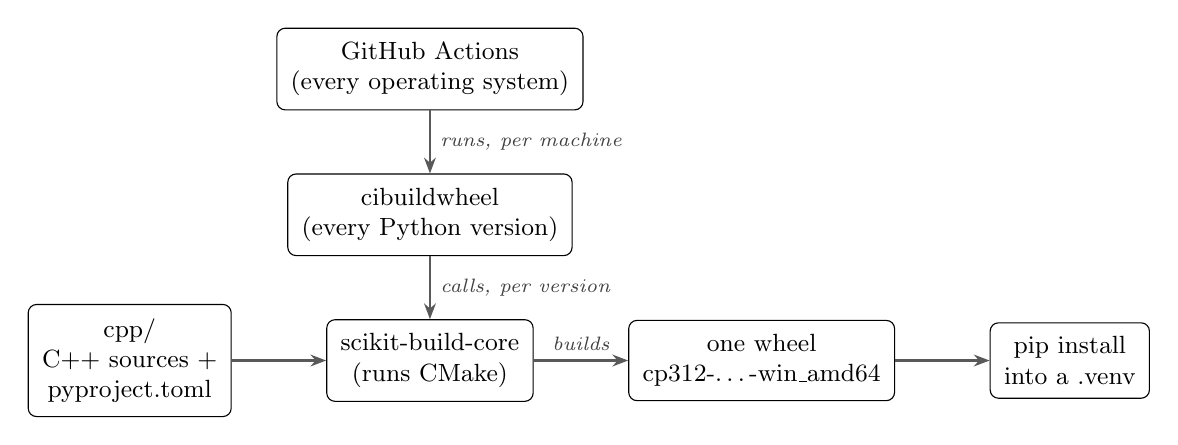
\begin{tikzpicture}[
  box/.style={draw, rounded corners=3pt, align=center, font=\small, inner sep=5pt, fill=white},
  arrow/.style={-{Stealth[length=2mm]}, thick, gray!70!black},
  lbl/.style={font=\scriptsize\itshape, gray!50!black}]
  \node[box] (src) {\code{cpp/}\\C++ sources +\\\code{pyproject.toml}};
  \node[box, right=12mm of src] (skb) {scikit-build-core\\(runs CMake)};
  \node[box, right=12mm of skb] (whl) {one wheel\\\code{cp312-\dots-win\_amd64}};
  \node[box, above=8mm of skb] (cibw) {cibuildwheel\\(every Python version)};
  \node[box, above=8mm of cibw] (gha) {GitHub Actions\\(every operating system)};
  \node[box, right=12mm of whl] (pip) {pip install\\into a \code{.venv}};
  \draw[arrow] (src) -- (skb);
  \draw[arrow] (skb) -- node[lbl, above]{builds} (whl);
  \draw[arrow] (whl) -- (pip);
  \draw[arrow] (cibw) -- node[lbl, right]{calls, per version} (skb);
  \draw[arrow] (gha) -- node[lbl, right]{runs, per machine} (cibw);
\end{tikzpicture}
\end{center}

\begin{center}\small
\begin{tabularx}{\linewidth}{@{}l X@{}}
\toprule
File & Role \\
\midrule
\code{cpp/pyproject.toml} & what the package is and how to build it (scikit-build-core) and how to
  build all variants (cibuildwheel) \\
\code{cpp/bindings/CMakeLists.txt} & the extension modules and what goes into the wheel \\
\code{cpp/scripts/build\_wheels.sh}, \code{.ps1} & all wheels of \emph{this} machine (macOS/Linux,
  Windows) \\
\code{.github/workflows/wheels.yml} & all wheels of \emph{all} machines, in GitHub's cloud \\
\code{python/scripts/setup\_env.sh}, \code{.ps1} & installs a wheel into the Python project \\
\bottomrule
\end{tabularx}
\end{center}

%==============================================================================
\part{Wheels}

\section{Anatomy of a wheel}

A wheel is a \textbf{zip file} with the extension \code{.whl}. Look inside one:
\begin{lstlisting}[language=bash]
$ python -m zipfile -l dist/nabia_python_bridge-0.1.0-cp314-cp314-macosx_13_0_arm64.whl
nabia_python_bridge/__init__.py
nabia_python_bridge/frames.py                       ... and the other .py files
nabia_python_bridge/_core.cpython-314-darwin.so     the whole C++ library, compiled
nabia_python_bridge/_rb_backtest.cpython-314-darwin.so
nabia_python_bridge-0.1.0.dist-info/METADATA        name, version, dependencies, README
nabia_python_bridge-0.1.0.dist-info/WHEEL           wheel format and tags
nabia_python_bridge-0.1.0.dist-info/RECORD          every file with its SHA-256 hash and size
\end{lstlisting}
\begin{itemize}
  \item The files are laid out \emph{exactly as they will be installed}: installing is unzipping
        into \code{site-packages}. Nothing is compiled at install time.
  \item \code{METADATA} lists the dependencies (\code{Requires-Dist: numpy>=1.24}), which pip
        installs too.
  \item \code{WHEEL} says \code{Root-Is-Purelib: false} (it contains compiled code) and repeats
        the tag.
  \item \code{RECORD} lets pip verify the files and uninstall them later.
\end{itemize}

\subsection{The filename is the compatibility contract}
\begin{center}
\code{nabia\_python\_bridge}\,-\,\code{0.1.0}\,-\,\code{cp314}\,-\,\code{cp314}\,-\,\code{macosx\_13\_0\_arm64}\,.whl
\end{center}
\begin{center}\small
\begin{tabularx}{\linewidth}{@{}l l X@{}}
\toprule
Part & Name & Meaning \\
\midrule
\code{nabia\_python\_bridge} & distribution & the package name (\code{project.name}) \\
\code{0.1.0} & version & \code{project.version} \\
\code{cp314} & Python tag & which Python implementation and version can run it: CPython 3.14 \\
\code{cp314} & ABI tag & which binary interface the compiled code uses. \code{abi3} would mean
  the stable ABI (one wheel for many versions); pybind11 modules use the full API, so it is the
  version itself \\
\code{macosx\_13\_0\_arm64} & platform tag & operating system, its minimum version, and the
  architecture \\
\bottomrule
\end{tabularx}
\end{center}

Platform tags you will meet:
\begin{description}
  \item[\code{manylinux\_2\_28\_x86\_64}, \code{\_aarch64}] Linux with glibc 2.28 or newer (Debian
        10+, Ubuntu 20.04+, RHEL 8+). ``Many'' Linux distributions, because the wheel only uses
        libraries every one of them has, in versions at least that old. It is built inside an old
        Linux container on purpose: code compiled against an old glibc runs on newer ones, not the
        reverse.
  \item[\code{macosx\_13\_0\_arm64}, \code{\_x86\_64}] macOS 13 or newer, on Apple silicon or Intel.
        The number comes from \code{MACOSX\_DEPLOYMENT\_TARGET} at build time; it tells the compiler
        which macOS APIs it may use.
  \item[\code{win\_amd64}, \code{win\_arm64}] 64-bit Windows on Intel/AMD, or on ARM.
  \item[\code{any}] no compiled code. The Python projects \code{nabia} and \code{nabia\_webui} would
        produce \code{py3-none-any} wheels: one file for every platform.
\end{description}

\subsection{How pip chooses}
pip computes the list of tags the running interpreter supports, most specific first, and picks
the first wheel that matches. See the list with \cmd|python -m pip debug --verbose|. If no wheel
matches, pip falls back to the \textbf{sdist} (source distribution, a \code{.tar.gz} of the
sources) and compiles it, which needs CMake and a C++20 compiler on that machine. That is why
binary packages publish one wheel per platform and Python version: users then never compile.

\section{Building one wheel}

\subsection{The build interface: \texorpdfstring{\code{[build-system]}}{[build-system]}}
pip does not know CMake. Since PEP~517, a project declares a \emph{build backend} that pip calls
in a fresh, isolated environment:
\filepiece{pyproject-build-system}{toml}{\code{cpp/pyproject.toml}: which backend builds the wheel}
\begin{enumerate}
  \item pip (or \code{python -m build}, or \code{uv build}) creates a temporary virtual environment
        and installs \code{requires} into it: scikit-build-core and pybind11.
  \item It calls the backend's \code{build\_wheel()}.
  \item scikit-build-core configures and builds the CMake project, runs the CMake install step into
        a staging folder, and zips that folder into a wheel with its \code{dist-info}.
\end{enumerate}

\subsection{What the package is: \texorpdfstring{\code{[project]}}{[project]}}
\filepiece{pyproject-project}{toml}{\code{cpp/pyproject.toml}: package metadata (becomes \code{METADATA})}
\code{dependencies} are installed by pip with the wheel. Optional groups are installed only on
request, for example with \cmd|pip install "nabia_python_bridge[test]"|:
\filepiece{pyproject-project-optional-dependencies}{toml}{\code{cpp/pyproject.toml}: optional dependency groups}

\subsection{How CMake is driven: \texorpdfstring{\code{[tool.scikit-build]}}{[tool.scikit-build]}}
\filepiece{pyproject-tool-scikit-build}{toml}{\code{cpp/pyproject.toml}: scikit-build-core settings}
\begin{itemize}
  \item \code{cmake.source-dir} is the folder with the top \code{CMakeLists.txt}: \code{cpp/} itself.
  \item \code{wheel.packages = []}: scikit-build-core copies no Python folder by itself; CMake
        installs everything (below). This keeps development leftovers out of the wheel.
  \item \code{build-dir} keeps a build folder per wheel tag, so rebuilding is incremental.
  \item \code{sdist.exclude} keeps build folders and documentation out of the source package.
\end{itemize}
\filepiece{pyproject-tool-scikit-build-cmake-define}{toml}{\code{cpp/pyproject.toml}: CMake options for wheel builds}
These are ordinary CMake cache variables, as with \code{-D} on the command line: only the bindings
are built (no tests, apps, examples or PDFs), and static libraries are compiled as
position-independent code so they can be linked into a shared module on Linux.

\subsection{What goes into the wheel: CMake install rules}
\filepiece{bindings-cmake}{cmake}{\code{cpp/bindings/CMakeLists.txt}: the modules and the install rules}
\code{SKBUILD} is defined only when scikit-build-core runs CMake. Then the two modules and the
\code{.py} files are \code{install}ed to \code{nabia\_python\_bridge/}, which becomes that folder
inside the wheel. In a normal CMake build (CLion, preset \code{python-bridge}) the modules are
instead written next to the \code{.py} files, for debugging from the source tree.

\begin{note}{Static linking.}
nabia, iir1 and the app's parser are static libraries, and Eigen is header-only, so all of their
code is \emph{inside} \code{\_core}: the wheel needs only the system C++ runtime. A wheel that links
a shared library (say \code{libfoo.so}) must carry a copy; cibuildwheel's \emph{repair} step
(\S\ref{sec:cibw}) does that.
\end{note}

\subsection{Try it}
\begin{lstlisting}[language=bash]
python/.venv/bin/python -m pip wheel ./cpp --no-deps -w dist     # one wheel, this Python
MACOSX_DEPLOYMENT_TARGET=13.0 python/.venv/bin/python -m pip wheel ./cpp --no-deps -w dist
uv build --wheel --python 3.12 --out-dir dist cpp                # with uv, another Python
uv build --sdist --out-dir dist cpp                              # the source package
\end{lstlisting}

\section{Installing and using a wheel}

\begin{lstlisting}[language=bash]
python -m venv .venv                                    # an isolated environment
.venv/bin/pip install --no-index --find-links dist nabia_python_bridge
\end{lstlisting}
\begin{itemize}
  \item \code{--find-links dist} adds a folder of wheels as a source; \code{--no-index} turns PyPI
        off, so the package must come from that folder.
  \item pip picks the matching file, reads its dependencies, installs them, unzips the wheel into
        \code{.venv/lib/python3.x/site-packages/}, and keeps its \code{dist-info} there.
  \item \code{import nabia\_python\_bridge} finds the folder; \code{\_\_init\_\_.py} imports
        \code{\_core}, and the operating system's loader maps the \code{.so} into the process.
\end{itemize}

\paragraph{Same version, new build.} pip skips a package whose version is already installed. After
rebuilding the C++ code without changing the version, reinstall explicitly:
\cmd|pip install --force-reinstall --no-deps ...|. The setup scripts do that every time:
\filepiece{setup-env-sh}{bash}{\code{python/scripts/setup\_env.sh}: the wheel, then the project in editable mode}

\paragraph{Editable installs.} \cmd|pip install -e python| does not copy \code{python/nabia}: it
installs a pointer to the source folder, so edits are live. That is how \code{python/} and
\code{webui/} are installed, while the C++ arrives as a finished wheel.

%==============================================================================
\part{Many wheels}

\section{All Python versions on one machine}
On macOS and Linux, \code{build\_wheels.sh} loops over versions with uv, which downloads any
missing Python:
\filepiece{build-wheels-sh}{bash}{\code{cpp/scripts/build\_wheels.sh}}
The pattern is the same for every wheel: \emph{build in isolation, install into a clean
environment, run the tests against the installed copy, keep it only if they pass}. Testing the
installed wheel, from outside the source tree, is the point: it catches a file missing from the
wheel, which tests run on the sources would never see.

\section{cibuildwheel}\label{sec:cibw}
cibuildwheel automates exactly that loop, for every platform, and adds what portable wheels need.
For each \emph{build identifier} --- \code{cp312-manylinux\_x86\_64}, \code{cp313-macosx\_arm64},
\code{cp314-win\_amd64}, \dots --- it:
\begin{enumerate}
  \item gets that Python (on Linux, inside a \code{manylinux} Docker container; on macOS and
        Windows, official installers it downloads);
  \item builds the wheel through the backend, like \code{pip wheel};
  \item \textbf{repairs} it: on Linux \code{auditwheel} checks it only uses allowed system libraries
        and copies others in, then sets the \code{manylinux} tag; on macOS \code{delocate} does the
        same for \code{.dylib}s; on Windows nothing by default;
  \item installs it in a fresh environment with \code{test-extras} and runs \code{test-command};
  \item moves it to the output folder.
\end{enumerate}

\subsection{Configuration}
\filepiece{pyproject-tool-cibuildwheel}{toml}{\code{cpp/pyproject.toml}: which wheels, and how to test them}
\begin{itemize}
  \item \code{build} and \code{skip} are glob patterns over identifiers. Here: CPython 3.10--3.14;
        no musl Linux, no 32-bit.
  \item \code{\{project\}} is the folder cibuildwheel was started in (the repository root, so the
        Python project's tests are reachable); \code{\{package\}} would be \code{cpp/}.
  \item Any setting can be overridden by an environment variable: \code{CIBW\_BUILD},
        \code{CIBW\_ARCHS}, \code{CIBW\_TEST\_SKIP}, \dots{} The workflow and the PowerShell script
        use that.
\end{itemize}
\filepiece{pyproject-tool-cibuildwheel-linux}{toml}{Linux: the container image}
\filepiece{pyproject-tool-cibuildwheel-macos}{toml}{macOS: the oldest supported version}

\subsection{Running it yourself}
\begin{lstlisting}[language=bash]
pipx run cibuildwheel==4.3.4 --print-build-identifiers --platform linux cpp   # what would be built
pipx run cibuildwheel==4.3.4 --platform linux cpp       # Linux wheels, needs Docker running
pipx run cibuildwheel==4.3.4 --platform macos cpp       # on a Mac
CIBW_BUILD="cp312-*" pipx run cibuildwheel==4.3.4 --platform linux cpp   # one version only
\end{lstlisting}
On Windows, \code{build\_wheels.ps1} wraps the same call: it checks Visual Studio, Git and Python,
installs cibuildwheel in a private environment and runs it from the repository root.
\filepiece{build-wheels-ps1}{PowerShell}{\code{cpp/scripts/build\_wheels.ps1}}

%==============================================================================
\part{GitHub Actions}

\section{Concepts}

GitHub Actions runs commands on machines in GitHub's cloud when something happens in the
repository. The vocabulary:
\begin{description}
  \item[Workflow] a YAML file in \code{.github/workflows/}. GitHub reads every file there. It must be
        at the repository root (not in \code{cpp/}).
  \item[Event] what starts it: a push, a tag, a pull request, a schedule, or a manual start
        (\code{workflow\_dispatch}). A manual start requires the workflow to exist on the default
        branch.
  \item[Run] one execution of a workflow, with a number and a page (Actions tab).
  \item[Job] a unit of work on \emph{one fresh machine}. Jobs run in parallel unless one
        \code{needs} another. Nothing on disk survives from one job to the next.
  \item[Runner] the machine: \code{ubuntu-24.04}, \code{ubuntu-24.04-arm}, \code{macos-14} (Apple
        silicon), \code{windows-latest}, \dots{} A fresh virtual machine each time.
  \item[Step] one command (\code{run:}) or one reusable \textbf{action} (\code{uses:}) inside a job,
        executed in order. If a step fails, the job stops and fails.
  \item[Action] a packaged step published in a repository, used as \code{owner/repo@version}:
        \code{actions/checkout@v5} clones the repository, \code{pypa/cibuildwheel@v4.3.4} runs
        cibuildwheel, \code{actions/upload-artifact@v4} saves files.
  \item[Artifact] files a job uploads to the run, to download later or in another job: the way to
        pass wheels from the build jobs to the collect job, and to you.
  \item[Matrix] one job definition expanded into several jobs, one per combination of values.
\end{description}

\subsection{YAML and expressions}
YAML is indentation-based: two spaces per level, \code{key: value}, lists with \code{- }, and
\code{\{ a: 1, b: 2 \}} as a one-line map. Text between \lstinline|${{| and \lstinline|}}| is an
\emph{expression} GitHub evaluates before running anything:
\begin{center}\small
\begin{tabularx}{\linewidth}{@{}l X@{}}
\toprule
Expression & Value \\
\midrule
\code{\$\{\{ matrix.os \}\}} & the current matrix value \\
\code{\$\{\{ github.ref \}\}} & what triggered the run: \code{refs/heads/main}, \code{refs/tags/v0.1.0} \\
\code{\$\{\{ github.token \}\}} & a temporary token for this run, with the job's \code{permissions} \\
\code{\$\{\{ secrets.NAME \}\}} & a secret set in Settings $\to$ Secrets and variables $\to$ Actions \\
\code{\$\{\{ needs.collect.result \}\}} & \code{success}, \code{failure}, \code{cancelled} or \code{skipped} \\
\code{startsWith(a, b)}, \code{!cancelled()} & functions and status checks, used in \code{if:} \\
\bottomrule
\end{tabularx}
\end{center}
Inside \code{run:} scripts, the same information is in environment variables
(\code{\$GITHUB\_REF\_NAME}, \code{\$GITHUB\_REPOSITORY}, \dots).

\section{nabia's workflow, piece by piece}

\subsection{Name and triggers}
\filepiece{workflow-head}{yaml}{\code{.github/workflows/wheels.yml}: when it runs}
\begin{itemize}
  \item \code{workflow\_dispatch}: the ``Run workflow'' button and \cmd|gh workflow run wheels.yml|.
  \item \code{push: tags: ["v*"]}: pushing a tag such as \code{v0.1.0}. Pushing commits to
        \code{main} does \emph{not} start it (no \code{branches:} filter is given).
  \item \code{pull\_request: paths:}: only pull requests that change those files.
\end{itemize}

\subsection{The build matrix}
\filepiece{job-wheels}{yaml}{The \code{wheels} job: one machine per platform}
\begin{itemize}
  \item \code{strategy.matrix.include} lists five combinations, so this definition becomes five
        jobs running in parallel, each with its own \lstinline|${{ matrix.os }}| and
        \lstinline|${{ matrix.archs }}|.
  \item \code{fail-fast: false}: a failure on one platform does not cancel the others.
  \item \code{runs-on} picks the machine from the matrix.
  \item Steps: clone the repository; run cibuildwheel on \code{cpp} (the action installs it and
        passes \code{with:} values as options and \code{env:} values as \code{CIBW\_*} settings);
        upload the wheels as an artifact named after the platform. Each runner builds the five
        Python versions of its platform.
  \item \code{macos-14} is an Apple silicon machine; the \code{x86\_64} entry cross-compiles Intel
        wheels there and tests them under Rosetta.
\end{itemize}

\subsection{Collecting everything}
\filepiece{job-collect}{yaml}{The \code{collect} job: every wheel and the sdist in one artifact}
\begin{itemize}
  \item \code{needs: wheels} waits for all five build jobs.
  \item By default a job runs only if everything it needs succeeded. \lstinline|if: ${{ !cancelled() }}|
        overrides that: it runs even if a platform failed, so the good wheels are not lost.
  \item \code{download-artifact} with \code{pattern} and \code{merge-multiple} puts the files of all
        \code{wheels-*} artifacts into one folder.
  \item \code{pipx run build --sdist} builds the source package, the fallback for platforms without
        a wheel.
\end{itemize}

\subsection{Publishing a release}
\filepiece{job-release}{yaml}{The \code{release} job: a GitHub Release on version tags}
\begin{itemize}
  \item The \code{if:} makes it run only for tags starting with \code{v}, and only if collecting
        succeeded. On manual runs it shows as \emph{skipped}.
  \item \code{permissions: contents: write}: the run's token is read-only by default; creating a
        release needs write access, granted to this job only.
  \item \code{gh} (the GitHub CLI, installed on every runner) creates the release with all files
        attached and notes generated from the commits since the previous tag.
\end{itemize}

\subsection{Testing the Windows scripts}
\filepiece{job-windows-script}{yaml}{The \code{windows-script} job}
\code{actions/setup-python} installs a Python and puts it on the \code{PATH};
\code{shell: pwsh} runs the steps with PowerShell. The job builds one wheel with
\code{build\_wheels.ps1}, installs it with \code{setup\_env.ps1}, and runs the Python project's
tests: the scripts a Windows user would run, run on Windows.

%==============================================================================
\part{Doing it yourself}

\section{Writing a job}
A recipe:
\begin{enumerate}
  \item \textbf{Pick the machine} (\code{runs-on}), or several with a matrix.
  \item \textbf{Start with \code{actions/checkout}}: a runner starts empty.
  \item \textbf{Install what is missing}: \code{actions/setup-python} for a given Python; compilers,
        CMake, Git and \code{gh} are preinstalled on GitHub's images.
  \item \textbf{Run commands} with \code{run:}, one step per logical action, each with a
        \code{name:} so the log reads well. Use \code{working-directory:} instead of \code{cd}.
  \item \textbf{Keep results} with \code{upload-artifact}; get them in another job with
        \code{needs:} and \code{download-artifact}.
  \item \textbf{Grant only the permissions needed}, per job.
\end{enumerate}
The examples below are not in the workflow; paste them under \code{jobs:} to use them.

\subsection{Example: the C++ tests on Linux and macOS}
\begin{lstlisting}[language=yaml]
  cpp-tests:
    name: C++ tests ${{ matrix.os }}
    strategy:
      fail-fast: false
      matrix:
        os: [ubuntu-24.04, macos-14]
    runs-on: ${{ matrix.os }}
    defaults:
      run:
        working-directory: cpp
    steps:
      - uses: actions/checkout@v5
      - name: Configure
        run: cmake --preset release -DNABIA_BUILD_DOCS=OFF
      - name: Build
        run: cmake --build --preset release -j 4
      - name: Test
        run: ctest --preset release
\end{lstlisting}
A list under \code{matrix} (\code{os: [a, b]}) is the short form of \code{include}; with several
lists, the matrix is their cross product.

\subsection{Example: the Python project's tests against the Linux wheel}
\begin{lstlisting}[language=yaml]
  python-tests:
    needs: wheels
    runs-on: ubuntu-24.04
    steps:
      - uses: actions/checkout@v5
      - uses: actions/setup-python@v5
        with:
          python-version: "3.12"
      - uses: actions/download-artifact@v4
        with:
          name: wheels-ubuntu-24.04-x86_64
          path: dist
      - name: Install the wheel and nabia
        run: PYTHON=python python/scripts/setup_env.sh
      - name: Tests
        working-directory: python
        run: .venv/bin/python -m pytest -q
\end{lstlisting}

\subsection{Example: publishing to PyPI without a password}
PyPI's \emph{trusted publishing} lets a workflow upload without storing a token: on pypi.org, under
the project's Publishing settings, register this repository, the workflow file \code{wheels.yml}
and an environment name (\code{pypi}). Then:
\begin{lstlisting}[language=yaml]
  pypi:
    needs: collect
    if: ${{ startsWith(github.ref, 'refs/tags/v') }}
    runs-on: ubuntu-24.04
    environment: pypi              # optional approval rules live in Settings > Environments
    permissions:
      id-token: write              # proves to PyPI which workflow is uploading
    steps:
      - uses: actions/download-artifact@v4
        with:
          name: all-wheels
          path: dist
      - uses: pypa/gh-action-pypi-publish@release/v1
\end{lstlisting}
Every upload needs a new version number in \code{cpp/pyproject.toml}: PyPI never accepts the same
version twice. Try it first on test.pypi.org (\code{with: repository-url:
https://test.pypi.org/legacy/}).

\subsection{Useful extras}
\begin{lstlisting}[language=yaml]
concurrency:                       # top level: a new run of the same branch cancels the older one
  group: wheels-${{ github.ref }}
  cancel-in-progress: true

    timeout-minutes: 60            # in a job: stop a hung job early (default 360)

      - uses: actions/cache@v4     # in steps: reuse downloads between runs
        with:
          path: ~/.cache/pip
          key: pip-${{ runner.os }}-${{ hashFiles('cpp/pyproject.toml') }}
\end{lstlisting}

\section{Running, watching and debugging}

\subsection{From the terminal}
\begin{center}\small
\begin{tabularx}{\linewidth}{@{}l X@{}}
\toprule
Command & Does \\
\midrule
\code{gh workflow run wheels.yml} & starts a run (the file must be on \code{main}) \\
\code{gh run list --workflow wheels.yml} & recent runs with their ids and status \\
\code{gh run watch \textless{}id\textgreater{}} & live status until it finishes \\
\code{gh run view \textless{}id\textgreater{}} & jobs and their results \\
\code{gh run view \textless{}id\textgreater{} --log-failed} & the log lines of failed steps (after the run ends) \\
\code{gh run rerun \textless{}id\textgreater{} --failed} & reruns only the failed jobs \\
\code{gh run cancel \textless{}id\textgreater{}} & stops a run \\
\code{gh run download \textless{}id\textgreater{} -n all-wheels -D dist} & downloads an artifact \\
\code{gh release list}, \code{gh release view v0.1.0} & releases and their files \\
\bottomrule
\end{tabularx}
\end{center}

\subsection{On the web}
Repository $\to$ \textbf{Actions} tab $\to$ \emph{wheels} in the sidebar $\to$ a run. The summary
page shows the jobs as a graph (\code{wheels} $\to$ \code{collect} $\to$ \code{release}) and, at the
bottom, the \textbf{Artifacts}. Click a job, then a step, to read its log; the gear menu downloads
the full log. \emph{Re-run jobs} and \emph{Cancel workflow} are at the top right.

\subsection{Reading a failure}
cibuildwheel ends a failed build with a summary such as
\begin{lstlisting}
Error: cibuildwheel: Command [... '-m', 'build', '.../cpp', '--wheel', ...] failed with code 1.
\end{lstlisting}
which only says \emph{that} the build failed. The cause is above it: search the log for
\code{error:} (compiler), \code{CMake Error}, \code{FAILED:} (the file that did not compile) or a
Python traceback. Failures met while setting up this workflow, and their fixes:
\begin{center}\small
\begin{tabularx}{\linewidth}{@{}>{\raggedright\arraybackslash}X >{\raggedright\arraybackslash}X >{\raggedright\arraybackslash}X@{}}
\toprule
Log & Cause & Fix \\
\midrule
\code{HTTP 404: workflow wheels.yml not found on the default branch} & the file was not pushed to
  \code{main} & commit and push it \\
\code{AssertionError: uv not found} (macOS, Windows) & \code{build-frontend = "build[uv]"} needs uv
  on the runner & use the default frontend \\
\code{error: no member named 'jthread' in namespace 'std'} & the Xcode 15 libc++ of \code{macos-14}
  is older than the local one & a joining \code{std::thread} wrapper \\
\code{'from\_chars' is unavailable: introduced in macOS 26.0} & a deployment target older than the
  library function & \code{strtod}/\code{snprintf} \\
\code{The run was canceled by @user} & cancelled by hand & nothing; rerun if needed \\
\bottomrule
\end{tabularx}
\end{center}
\begin{note}{Reproduce locally first.}
A CI round trip takes minutes; most failures reproduce on your machine:
\cmd|cpp/scripts/build_wheels.sh 3.12| for macOS, \cmd|pipx run cibuildwheel --platform linux cpp|
with Docker for Linux, an older \code{MACOSX\_DEPLOYMENT\_TARGET} for macOS availability errors.
\end{note}

\section{Releasing}
\begin{center}\small
\begin{tabularx}{\linewidth}{@{}l >{\raggedright\arraybackslash}X >{\raggedright\arraybackslash}X@{}}
\toprule
Where & Who can install & How \\
\midrule
Run artifacts & you and collaborators, logged in, for 90 days & \code{gh run download} \\
GitHub Release & anyone who can see the repository (it is private: collaborators); permanent &
  \code{git tag v0.1.0 \&\& git push origin v0.1.0}, then download from the Releases page \\
PyPI & anyone: \code{pip install nabia-python-bridge} & trusted publishing job, new version each time \\
\bottomrule
\end{tabularx}
\end{center}
A release checklist:
\begin{enumerate}
  \item Set the version in \code{cpp/pyproject.toml} (and in \code{python/} and \code{webui/} if they
        are published too); commit and push.
  \item Start a manual run and check every job is green.
  \item Tag and push the tag: \cmd|git tag v0.2.0 && git push origin v0.2.0|. The tag run builds
        again and creates the release.
\end{enumerate}

\section{Costs and limits}
\begin{itemize}
  \item \textbf{Minutes.} The repository is private, so runs use the account's included Actions
        minutes, and macOS and Windows minutes count more than Linux ones (see Settings $\to$
        Billing). A full run builds 25 wheels on five machines plus the Windows script job; trigger
        it when needed rather than on every push.
  \item \textbf{Storage.} Artifacts count toward the account's storage until they expire (90 days
        by default); releases do not expire.
  \item \textbf{Versions.} Pin actions to versions (\code{@v5}, \code{@v4.3.4}) so a new release of an
        action cannot change the build unannounced; update them deliberately.
\end{itemize}

\appendix
\section{Glossary}
\begin{description}\small
  \item[ABI] application binary interface: how compiled code calls other compiled code. CPython's
        changes between minor versions.
  \item[auditwheel, delocate, delvewheel] tools that copy shared libraries into a wheel and fix its
        tag (Linux, macOS, Windows).
  \item[build backend / frontend] the backend (scikit-build-core) turns a project into a wheel; the
        frontend (pip, \code{build}, \code{uv build}) calls it in an isolated environment.
  \item[deployment target] the oldest macOS a binary supports.
  \item[editable install] an install that points to the source folder instead of copying it.
  \item[glibc] the GNU C library of Linux; \code{manylinux\_2\_28} means version 2.28 or newer.
  \item[sdist] source distribution: the sources and \code{pyproject.toml}, compiled on install.
  \item[site-packages] the folder of an environment where packages are installed.
  \item[wheel tag] the \code{python-abi-platform} part of a wheel's name.
\end{description}

\end{document}
